\newpage % Rozdziały zaczynamy od nowej strony.
\cleardoublepage % Zaczynamy od nieparzystej strony
\pagestyle{headings}

\section{Wyniki i wnioski}
Celem pracy było zbadanie wpływu zastosowania akceleratorów, realizowanych w~technice HLS na szybkość działania algorytmów ANN.
W projekcie zaimplementowano i przetestowano kilka różnych modeli Sztucznych Sieci Neuronowych, klasyfikujących odręcznie pisane cyfry. Aby porównać rozwiązanie, realizowane w technice HLS z implementacją przy użyciu pakietu \emph{keras}, uruchamianą na komputerze PC każdy z modeli poddano testom, które zostały podzielone na następujące części:
\begin{itemize}
  \item uruchomienie sieci przy użyciu zbioru testowego 10000 cyfr z bazy MNIST, w celu oszacowania dokładności i 
  szybkości działania algorytmu.
  \item test wykonany w czasie rzeczywistym przy użyciu modułu kamery
  \item zbadanie wpływu optymalizacji w narzędziu Vivado HLS.
\end{itemize}
Zbadano wpływ różnych rozwiązań optymalizacji w narzędziu Vivado HLS na szybkość wykonywanych obliczeń oraz zajętość zasobów układu FPGA.
Wyniki testów z nich zamieszczone są w dalszej części rozdziału.

\subsection{Test modelu sieci z jedną warstwą ukrytą}

Model Sztucznej Sieci Neuronowej z jedną warstwą ukrytą zaimplementowano w~skrypcie pythona z użyciem biblioteki \emph{keras}. Wykonano uczenie sieci w 20 epokach z~wielkością mini-serii równą 128.
Model poddany testom w każdym z neuronów zawierał funkcję aktywacji \emph{sigmoid} i składał się z następujących warstw: 
\begin{itemize}
  \item warstwa wejściowa (784 wejścia)
  \item warstwa ukryta (16 neuronów)
  \item warstwa wyjściowa (10 neuronów).
\end{itemize}

Test z użyciem akceleratora HLS wykonano, podając na wejście sieci 10000 obrazów zapisanych w postaci plików tekstowych, zawierających po 784 wartości w przedziale od 0 do 1. Wynik testu, widoczny na Rys. \ref{wynik1} potwierdził poprawność działania algorytmu. Osiągnięto dokładność na poziomie 94,97\%, co pokrywa się z wynikiem uzyskanym z~wykorzystaniem biblioteki \emph{keras}, na komputerze PC.

\begin{figure}[!h]
    \centering
    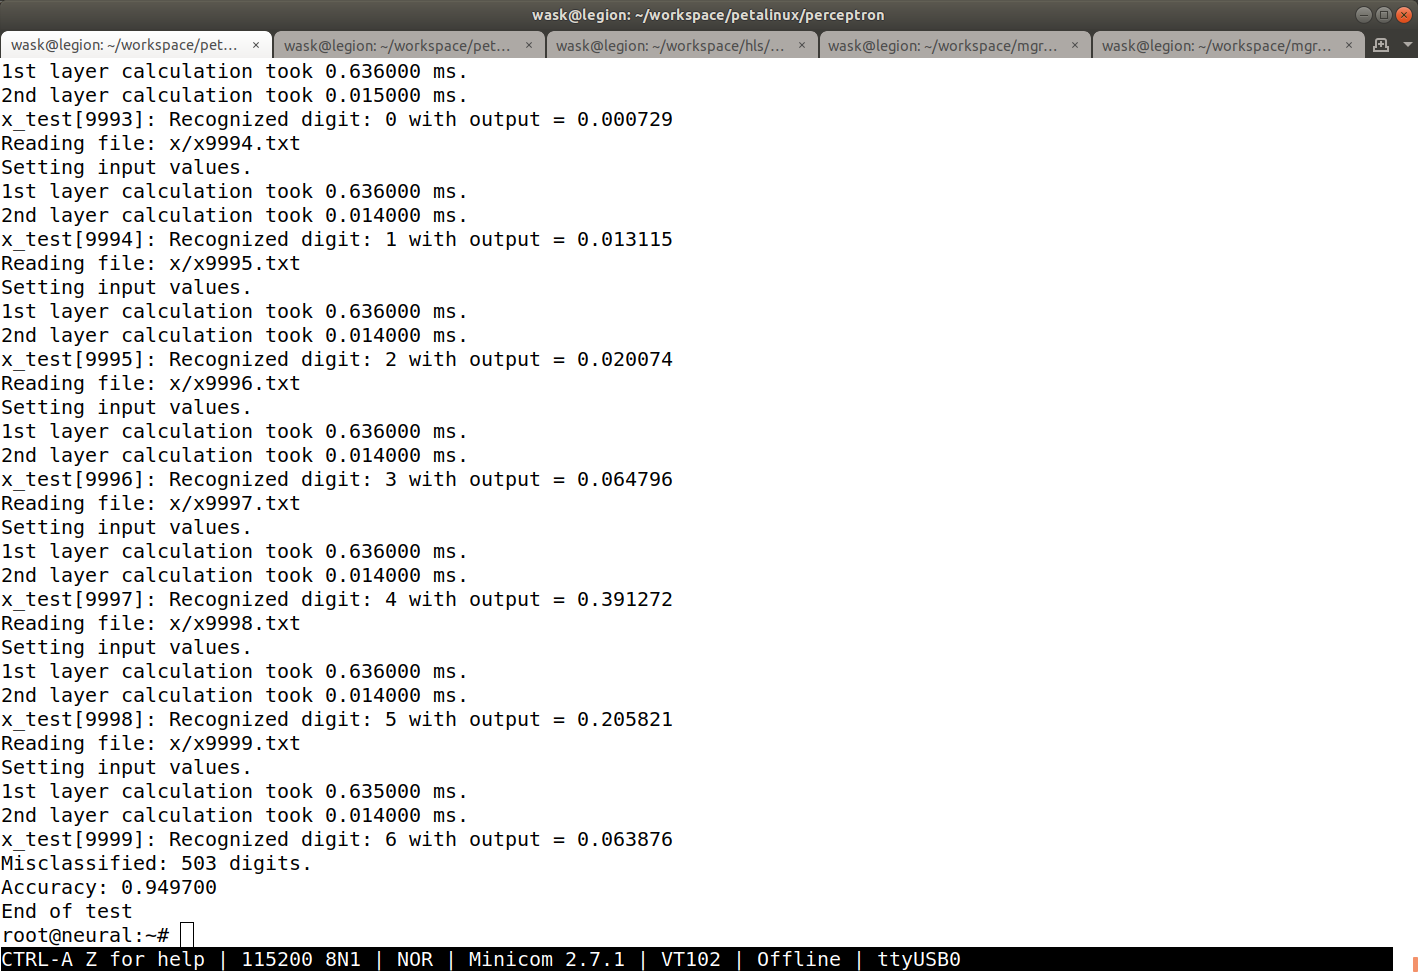
\includegraphics[width=\textwidth]{img/wynik1.png}
    \caption{Wynik testu uruchomionego na SBC Z-turn -- ANN z jedną warstwą ukrytą}
    \label{wynik1}
  \end{figure}


\subsubsection{Test klasyfikacji cyfr z użyciem kamery}

Następnym krokiem był test przeprowadzony w czasie rzeczywistym z użyciem kamery. Rozpoznawanie obiektów na obrazie w czasie rzeczywistym podzielono na 3 części:
\begin{itemize}
    \item detekcja kształtów przypominających cyfry i odrzucenie niewłaściwych obiektów
    \item przygotowanie obrazów do klasyfikacji (odpowiedni rozmiar obrazu i padding)
    \item klasyfikacja obrazów przy użyciu ANN
\end{itemize}

Pierwszą symulację wykonano na komputerze PC przy użyciu biblioteki OpenCV i pakietu \emph{keras}.
Ze względu na sporą ilość obliczeń początkowo zdecydowano się na zarejestrowanie obrazu oraz 
detekcję cyfr przy użyciu biblioteki OpenCV. 

Obraz był rejestrowany przy użyciu funkcji \emph{cv2.VideoCapture()} w rozdzielczości 640$\times$480 pikseli. 
Następnym krokiem było przekształcenie barwy obrazu na skalę szarości, rozmycie obrazu oraz 
za pomocą funkcji \emph{cv2.adaptiveThreshold} przekształcenie w obraz binarny z odwróconymi 
kolorami. Istotne jest, żeby obraz zawierał białą cyfrę na czarnym tle, ponieważ takie obrazy były 
w zbiorze uczącym.  Następnie użyto funkcji \emph{cv2.findContours}, która zwraca współrzędne 
prostokątów, w które wpisane są kontury znalezione przez algorytm. Po wyeliminowaniu niewłaściwych 
konturów można przejść do przygotowania obrazów do klasyfikacji. 

\begin{figure}[!h]
    \centering
    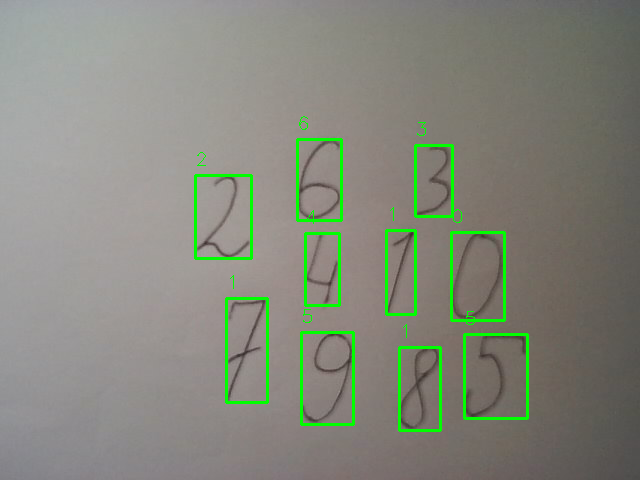
\includegraphics[width=\textwidth]{img/1hid-layer-pc-img.png}
    \caption{Ramka obrazu podczas testu ANN z jedną warstwą ukrytą uruchomionego na PC}
    \label{1hid-layer-pc-img}
  \end{figure}

Odpowiednio przycięty do rozmiaru 28$\times$28 pikseli i wycentrowany obraz ręcznie pisanej cyfry może 
zostać poddany klasyfikacji za pomocą nauczonego wcześniej modelu ANN. W wyniku testu otrzymano 
wyniki przedstawione na Rys. \ref{1hid-layer-pc-img}. 

\begin{figure}[!h]
    \centering
    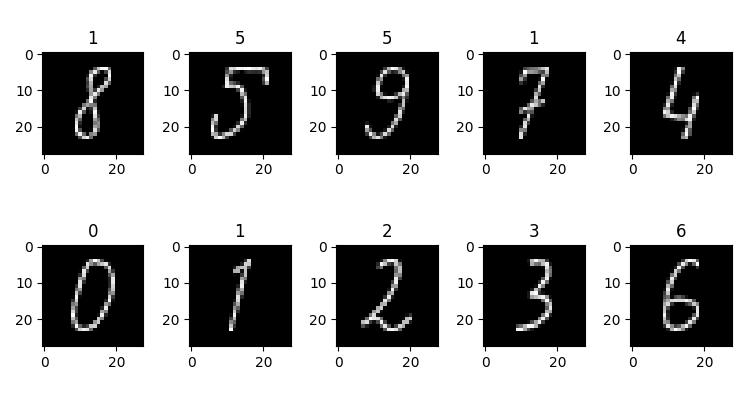
\includegraphics[width=\textwidth]{img/1hid-layer-pc-plot.png}
    \caption{Wynik testu ANN z jedną warstwą ukrytą uruchomionego na PC}
    \label{1hid-layer-pc-plot}
\end{figure}


Rysunek Rys. \ref{1hid-layer-pc-plot} zawiera znalezione na obrazie cyfry i wynik klasyfikacji (nad 
każdą z cyfr). Widać, że 3 z 10 cyfr zostały sklasyfikowane nieprawidłowo, co daje dokładność 
klasyfikacji sieci 70\%.

\subsubsection{Test na płytce Z-turn z użyciem kamery}

W teście na płytce Z-turn zastosowano metodę rejestrowania obrazu taką jak na komputerze PC, jednak 
do rozpoznania cyfr wykorzystano akcelerator obliczeń ANN zaimplementowany w układzie FPGA.  
Aby umożliwić użytkownikowi wyświetlanie obrazu w czasie rzeczywistym, wykorzystano pakiety \emph{pickle} i \emph{socket} do wysyłania kolejnych ramek obrazu przez protokół TCP (ang. \emph{Transmission Control Protocol}). Aplikacja \emph{camera\_server.py} po uruchomieniu na płytce Z-turn oczekuje na połączenie pod zadanym adresem IP 10.42.0.1. Uruchomienie aplikacji \emph{camera\_client} na komputerze PC podłączonym z płytką przy użyciu kabla \emph{Ethernet} powoduje rozpoczęcie rejestrowania obrazu, detekcję i zapisanie obrazów przedstawiających cyfry do plików tekstowych. Działający w tle sterownik UIO \emph{rtdigitrecognition} zawiera mechanizm \emph{inotify}, pozwalający na monitorowanie zmian w~pliku \emph{input.txt}, zawierającym dane wejściowe sieci i reagowanie w przypadku zapisania nowych danych. Wynik klasyfikacji odręcznie pisanej cyfry jest zapisywany do pliku \emph{out.txt} i odczytywany w aplikacji rejestrującej obraz, w celu wyświetlenia wyniku przy odpowiedniej cyfrze. Wynik testu przedstawiono na Rys. \ref{1hid-layer-zturn-img}.

\begin{figure}[!h]
    \centering
    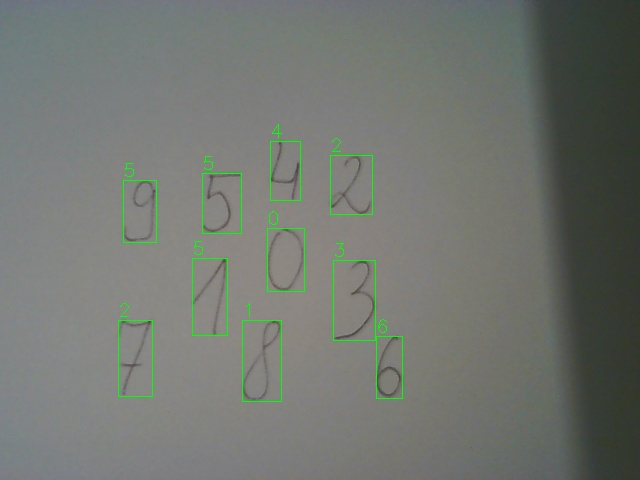
\includegraphics[width=\textwidth]{img/1hid-layer-zturn-img.jpg}
    \caption{Wynik testu ANN z jedną warstwą ukrytą uruchomionego na płytce Z-turn Board}
    \label{1hid-layer-zturn-img}
\end{figure}

Po otrzymaniu wyników pierwszego testu podjęto decyzję o modyfikacji modelu Sztucznej Sieci 
Neuronowej. Pierwszą zmianą było dodanie kolejnej warstwy ukrytej.

\subsection{Test modelu posiadającego dwie warstwy ukryte}

Dodano do istniejącego modelu kolejną warstwę ukrytą zawierającą 64 neurony. Po wykonaniu 50 epok uczenia 
sieci otrzymano dokładność na poziomie 97,17\%. Wykres z~przebiegu uczenia sieci przedstawiający dokładność 
klasyfikacji w kolejnych epokach przedstawiono na Rys. \ref{keras-accuracy2}. Na wykresie widać, że dokładność
po 20 epoce uczenia przestaje rosnąć, więc zwiększanie liczby epok nie da lepszych rezultatów i może prowadzić do 
przeuczenia sieci.   

\begin{figure}
    \centering
    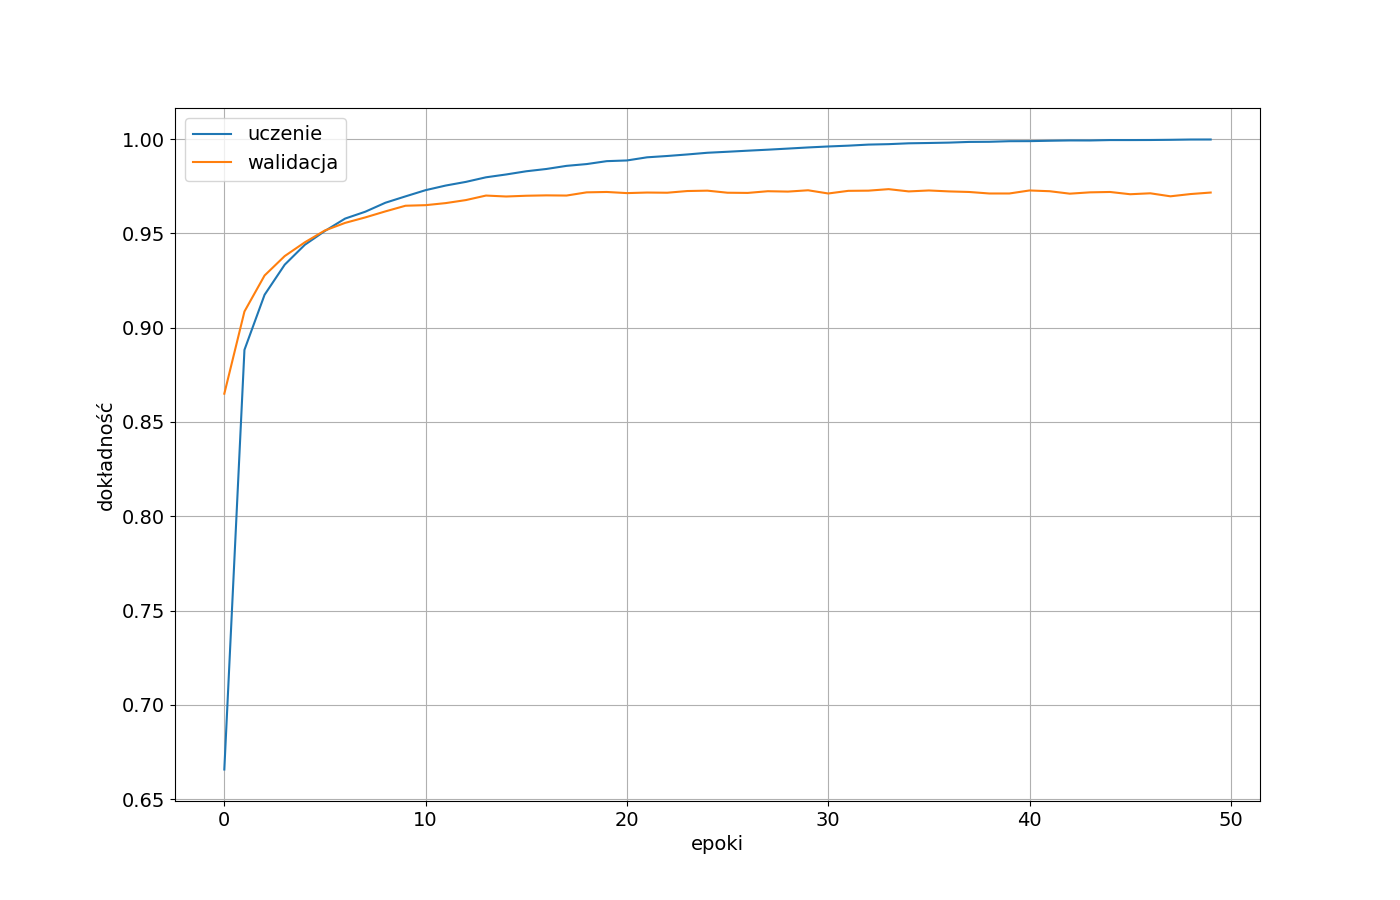
\includegraphics[width=\textwidth]{img/keras-accuracy2.png}
    \caption{Wykres zmian dokładności w kolejnych epokach -- ANN z dwoma warstwami ukrytymi}
    \label{keras-accuracy2}
\end{figure}


\subsection{Implementacja akceleratora obliczeń ANN w Vivado HLS}
  Parametry modelu sieci ANN stworzonego, nauczonego i przetestowanego w skrypcie Pythona z użyciem biblioteki keras są przekazywane do funkcji w Vivado HLS. Funkcja \emph{calcPerceptron()} jako argument przyjmuje następujące dane:
  \begin{itemize}
    \item dane wejściowe \emph{x} (obraz odręcznie pisanej cyfry)
    \item wagi sieci neuronowej \emph{w}
    \item biasy sieci neuronowej \emph{b}
    \item adres tablicy na dane wyjściowe sieci \emph{res}
    \item model sieci w postaci tablicy \emph{model} zawierającej:
    \begin{itemize}
      \item liczbę warstw sieci
      \item liczbę wejść sieci
      \item liczbę neuronów w każdej warstwie.
    \end{itemize}
  \end{itemize}

Zmieniając wartości tablicy \emph{model}, użytkownik może zmieniać parametry sieci z poziomu 
aplikacji. Ograniczeniami są rozmiary tablic zawierających parametry sieci, które muszą być 
ustalone na etapie tworzenia projektu oraz ilość pamięci BRAM w układzie \emph{Zynq}.
   
Ponadto z poziomu aplikacji użytkownik ma możliwość ustawienia parametru progu przycinania sieci 
(ang. \emph{pruning threshold}). Dzięki temu możliwe jest wyeliminowanie redundantnych wag sieci, które nie mają znacznego wpływu na wartość wyjścia sieci i~skrócenie obliczeń.


\subsection{Porównanie czasu wykonania różnych implementacji}

Aby przetestować wydajność klasyfikacji danego modelu sieci w implementacji programowej, uruchamianej na komputerze PC z użyciem pakietu \emph{keras}, wykorzystano metodę \emph{model.predict()}. Jako argument funkcja przyjmuje zbiór testowy z bazy MNIST.
Implementacja modelu w HLS z możliwością zmiany parametrów sieci nie dała zadowalających rezultatów. Wyniki dla różnych architektur sieci zestawiono w Tabeli \ref{tab:czas-wykonania}. 

\begin{table}[h] \centering
  \caption{Porównanie czasu wykonania implementacji software'owej przy użyciu pakietu keras z~implementacją w układzie FPGA z wykorzystaniem akceleratora HLS -- pierwsze podejście}
  \centering
  \begin{tabular} {c|c|c} \hline \label{tab:czas-wykonania}  
    implementowany model & aplikacja z użyciem keras & akcelerator HLS\\ \hline \hline
    FC10-sig-FC16-sig-FC16-sig-FC10-sig & 0.572 \emph{ms} & 0.635 \emph{ms} \\
    FC16-sig-FC10-sig & 0.569 \emph{ms} & 0.941 \emph{ms} \\
    FC64-sig-FC16-sig-FC10-sig & 0.535 \emph{ms} & 3.796 \emph{ms} \\
    FC16-sig-FC10-soft & 0.457 \emph{ms} & 0.938 \emph{ms} \\
    FC16-relu-FC10-soft & 0.435 \emph{ms} & 0.942 \emph{ms} \\
  \end{tabular}
\end{table}

Wykonanie klasyfikacji przy użyciu pakietu keras daje porównywalne wyniki dla każdego z testowanych modeli. W przypadku użycia sieci zawierającej dużą liczbę neuronów w pierwszej warstwie ukrytej czas wykonania obliczeń znacznie rośnie.



\subsection{Dostosowanie parametrów w implementacji HLS}

Implementacja umożliwiająca zmianę parametrów modelu sieci z poziomu aplikacji jest bardzo wygodnym 
rozwiązaniem, umożliwiającym szybkie przeprowadzenie testów dla różnych modeli sieci. Jednak 
zdefiniowanie w implementacji HLS parametrów sieci w~postaci zmiennych, spowodowało znaczne 
ograniczenia w możliwościach optymalizacji. 

\subsubsection{Optymalizacja pętli}

W przypadku optymalizacji pętli dwie najczęściej wykorzystywane dyrektywy to PIPELINE i LOOP UNROLL. Gdy pętla jest zagnieżdżona przy użyciu PIPELINE dodatkowo wykonywana jest dyrektywa LOOP FLATTEN, powodująca zamianę pętli zagnieżdżonej w pojedynczą pętlę. Wykonanie dyrektywy LOOP FLATTEN nie jest możliwe na pętli zagnieżdżonej, zawierającej zmienną w warunku zakończenia pętli wewnętrznej.

Pierwszym napotkanym problemem był brak możliwości pełnego rozwinięcia pętli przy użyciu dyrektywy:
\begin{verbatim}
  #pragma HLS UNROLL
\end{verbatim}
spowodowany zapisaniem warunku zakończenia pętli w zmiennej, będącej parametrem funkcji bloku HLS. 
W wyniku wykonania syntezy kompilator Vivado HLS zwracał komunikat informujący o braku możliwości pełnego rozwinięcia pętli.

Aby osiągnąć maksymalną akcelerację obliczeń i optymalizację zasobów zmieniono założenia projektu. Parametry modelu zostały ustalone na etapie implementacji bloku HLS. Dzięki temu możliwe było osiągnięcie znacznie lepszych wyników optymalizacji w~narzędziu Vivado HLS.

Następnym problemem związanym z rozwijaniem pętli był komunikat Vivado HLS o~braku możliwości wykonania operacji wczytania danych z jednej z tablic, spowodowany użyciem pamięci BRAM, posiadającej tylko dwa porty. Sugerowanym rozwiązaniem jest użycie innego bloku pamięci pozwalającego na równoległy odczyt dużej ilości danych lub partycjonowanie tablicy.

\subsubsection{Dobranie parametru \emph{II}}

Wykonano analizę wpływu zmian parametru \emph{II} dyrektywy PIPELINE na zajętość zasobów układu FPGA oraz czas wykonywania obliczeń. Pożądaną wartością tego parametru jest 1, jednak bywa, że wiąże się to z dużym zużyciem zasobów. W ramach kompromisu pomiędzy szybkością działania a zużyciem mocy można zmieniać parametr \emph{II}. Wyniki testów zamieszczono w Tabeli \ref{tab:ii-relu}.

\begin{table}[h] \centering
  \caption{Wpływ zmian parametru \emph{II} na wydajność systemu}
  \centering
  \begin{tabular} {c|c|c|c|c} \hline \label{tab:ii-relu}  

                  & \emph{II} = 1   & \emph{II} = 2   & \emph{II} = 3   & \emph{II} = 4   \\\hline
    opóźnienie    & 59.963  $\mu s$ & 68.630 $\mu s$  & 68.928 $\mu s$  & 70.606 $\mu s$  \\
    BRAM          & 5\%             & 4\%             & 4\%             & 4\%             \\
    DSP           & 15\%            & 10\%            & 9\%             & 8\%             \\
    FF            & 20\%            & 20\%            & 20\%            & 19\%            \\
    LUT           & 59\%            & 59\%            & 58\%            & 58\%            \\
  \end{tabular}
\end{table}


\subsection{Arytmetyka stałoprzecinkowa}

Kolejną metodą optymalizacji kodu jest zastosowanie arytmetyki stałoprzecinkowej. Przy użyciu typu \emph{ap\_fixed<W, I>} możliwe jest ustalenie liczby bitów przeznaczonych na część całkowitą \textbf{I} oraz liczby bitów \textbf{W}, przeznaczonej na całą zmienną. Ponadto biblioteka pozwala na ustalenie, co się stanie w przypadku przekroczenia maksymalnej lub minimalnej wartości, jaka może być reprezentowana przez ustaloną liczbę bitów.

W kodzie akceleratora HLS zaimplementowano oddzielne typy dla każdej ze zmiennych reprezentujących parametry sieci. Po wykonaniu analizy raportu dla różnych konfiguracji typów stałoprzecinkowych okazało się, że wprowadzenie arytmetyki stałoprzecinkowej w tym projekcie powoduje duże zużycie zasobów (ponad 100\%), przy nieznacznym spadku opóźnień. W związku z tym zdecydowano się na wykorzystanie typu zmiennoprzecinkowego.

Wykonano testy dla różnych typów wykorzystanych do deklaracji zmiennych w kodzie HLS. Użycie typu \emph{ap\_fixed} spowodowało zmniejszenie wprowadzanych opóźnień, ale liczba układów DSP urosła do wartości 362\%, co uniemożliwiło implementację tego rozwiązania. Dla każdego z typów najpierw uruchomiono symulację w Vivado HLS, aby sprawdzić poprawność wykonywanych obliczeń.
Typem o najmniejszej liczbie bitów, który dawał jeszcze poprawny wynik w symulacji był ap\_fixed<10,6>. Oprócz typów stałoprzecinkowych przetestowano również typy zmiennoprzecinkowe \emph{half} (16-bitowy) oraz \emph{float} (32-bitowy). Test wykonano na modelu zawierającym wszystkie funkcje aktywacji typu sigmoid.

\begin{table}[h] \centering
  \caption{Porównanie implementacji z wykorzystaniem różnych typów zmiennych}
  \centering
  \begin{tabular} {c|c|c|c|c|c} \hline \label{tab:fixed-vs-float}  
                  & float           & half            & ap\_fixed<12,7> & ap\_fixed<10,6> & ap\_fixed<16,7> \\ \hline
    opóźnienie    & 77.703 $\mu s$  & 78.063 $\mu s$  & 63,723 $\mu s$  & 63,723 $\mu s$  & 63,723 $\mu s$  \\
    BRAM          & 7\%             & 3\%             & 2\%             & 2\%             & 3\%             \\
    DSP           & 10\%            & 9\%             & \textbf{362\%}  & \textbf{362\%}  & \textbf{362\%}  \\
    FF            & 36\%            & 19\%            & 28\%            & 24\%            & 39\%            \\
    LUT           & 62\%            & 57\%            & 49\%            & 49\%            & 50\%            \\
    \emph{II}     & 4               & 4               & 4               & 4               &  4              \\
  \end{tabular}
\end{table}

W celu sprawdzenia, czy zajętość zasobów jest związana z obliczaniem funkcji sigmoid, powtórzono test na modelu zawierającym funkcje aktywacji ReLU oraz softmax w ostatniej warstwie. Wyniki przedstawiono w Tabeli \ref{tab:fixed-vs-float-relu}. Widać, że zmiana funkcji aktywacji nie miała znaczącego wpływu na zużycie zasobów układu FPGA. Czas wykonywania obliczeń dla typóœ zmiennoprzecinkowych jest nieco krótszy, lecz dla typów stałoprzecinkowych zużycie elementów DSP nadal przekracza 36\%.

\begin{table}[h] \centering
  \caption{Porównanie implementacji z wykorzystaniem różnych typów zmiennych -- funkcja aktywacji ReLU}
  \centering
  \begin{tabular} {c|c|c|c|c} \hline \label{tab:fixed-vs-float-relu}  
                  & float           & half            & ap\_fixed<12,7> & ap\_fixed<10,6> \\ \hline
    opóźnienie    & 58.306 $\mu s$  & 59.963 $\mu s$  & 75,750 $\mu s$  & 75,720 $\mu s$  \\
    BRAM          & 10\%             & 5\%             & 2\%             & 2\%            \\
    DSP           & 19\%            & 15\%             & \textbf{361\%}  & \textbf{361\%} \\
    FF            & 39\%            & 20\%            & 25\%            & 21\%            \\
    LUT           & 69\%            & 59\%            & 46\%            & 46\%            \\
    \emph{II}     & 1               & 1               & 1               & 1               \\
  \end{tabular}
\end{table}


\subsection{Wyniki po wykonaniu optymalizacji HLS}
Po wstępnych testach zdecydowano zmienić założenia implementacji i dokonać optymalizacji wybranej architektury sieci neuronowej. Do testów i optymalizacji w Vivado HLS wybrano model, składający się z następujących warstw:

\begin{itemize}
  \item warstwa wejściowa -- 784 wejścia sieci
  \item warstwa ukryta  -- 16 neuronów
  \item warstwa wyjściowa -- 10 neuronów
\end{itemize}

W każdym neuronie zastosowano funkcję aktywacji sigmoid. Wykonano uczenie sieci, stosując liczbę epok równą 20.
W wyniku testu sieci przy użyciu pakietu keras otrzymano dokładność klasyfikacji na poziomie 94,14\%.

Wybrany model, zawierający wszystkie funkcje aktywacji sigmoid, zaimplementowano w programie Vivado HLS. Ustalenie wartości parametrów liczby wejść i neuronów na etapie implementacji HLS dało większe możliwości optymalizacji. Raport z syntezy umieszczono na Rys. \ref{hls-report2}. Widać, że parametr II (ang. \emph{Initiation Interval}) jest duży i jest jeszcze możliwość optymalizacji algorytmu. Zużycie zasobów jest na akceptowalnym poziomie.

\begin{figure}[!h]
  \centering
  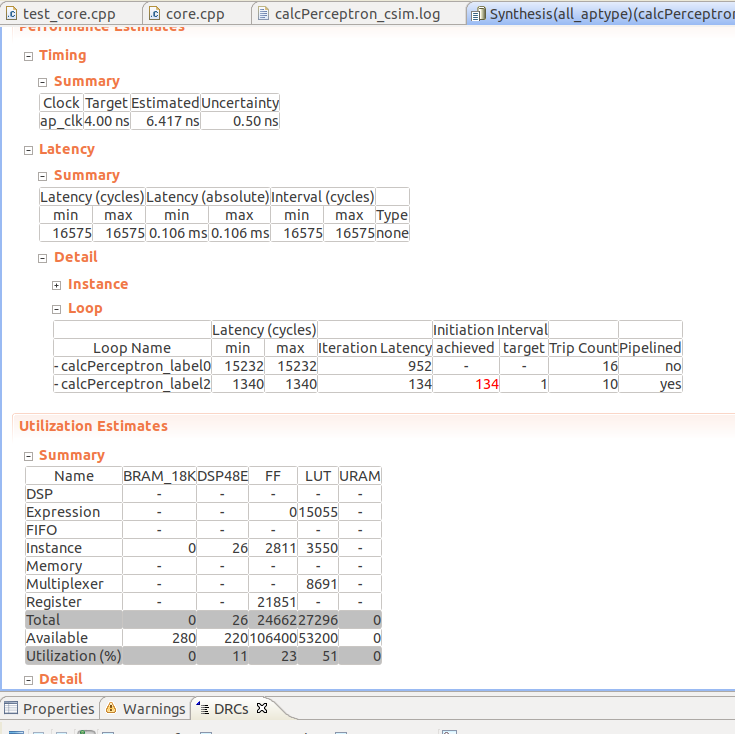
\includegraphics[width=\textwidth]{img/hls-report2.png}
  \caption{Raport po przeprowadzeniu syntezy w Vivado HLS -- drugie podejście}
  \label{hls-report2}
\end{figure}

W wyniku pierwszych testów otrzymano średni czas klasyfikacji jednego obrazu z~użyciem akceleratora HLS 
0.167110 \emph{ms}, a z zastosowaniem pakietu keras 0.463247~\emph{ms}. Daje to akcelerację obliczeń na 
poziomie 2,7.

Po przeanalizowaniu kodu i komunikatów kompilatora Vivado HLS zidentyfikowano problem, powodujący tak duży parametr II. Była to zależność niewłaściwie interpretowana przez kompilator Vivado HLS w pętli wykonującej obliczenia dla danego neuronu.

Aby osiągnąć \emph{II = 1} potrzebny był dodatkowy bufor przechowujący sumę iloczynów wejść i wag neuronu w danej iteracji. Dopiero po wyjściu z pętli, gdy sumy iloczynów są policzone dla każdego neuronu w danej warstwie, w kolejnej pętli liczona jest funkcja aktywacji każdego z neuronów. Takie podejście umożliwia osiągnięcie parametru \emph{II = 1}~dla obu pętli.

Osiągnięto parametr \emph{II = 1} jednak drastycznie wzrosło zużycie zasobów układu FPGA, co widać na Rys. \ref{hls-report3}.

\begin{figure}[!h]
  \centering
  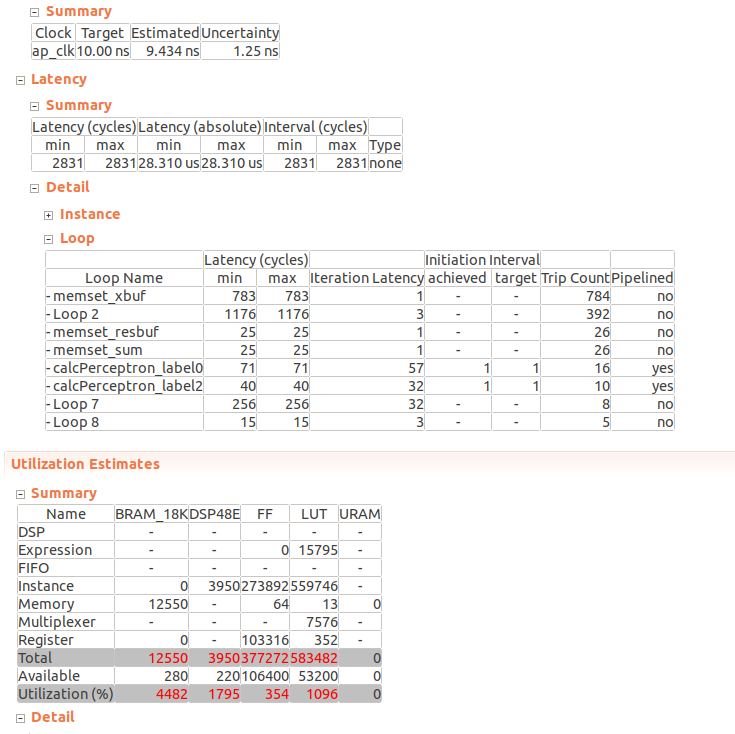
\includegraphics[width=\textwidth]{img/hls-report3.png}
  \caption{Raport po przeprowadzeniu syntezy w Vivado HLS -- minimalizowanie parametru II}
  \label{hls-report3}
\end{figure}

Zajętość elementów BRAM wyniosła ponad 4000\%, co wynika z użycia pamięci BRAM do przechowania całej tablicy zawierającej wagi sieci. Aby temu zapobiec, skorzystano z~dyrektywy RESOURCE, pozwalającej na wyspecyfikowanie, jakie zasoby będą użyte do zaimplementowania danej zmiennej. Zastosowano dyrektywę zapewniającą implementację tablicy wag jako dwuportową pamięć typu ROM:
\begin{verbatim}
  #pragma HLS RESOURCE variable=w core=ROM_2P_BRAM
\end{verbatim}


\begin{figure}[!h]
  \centering
  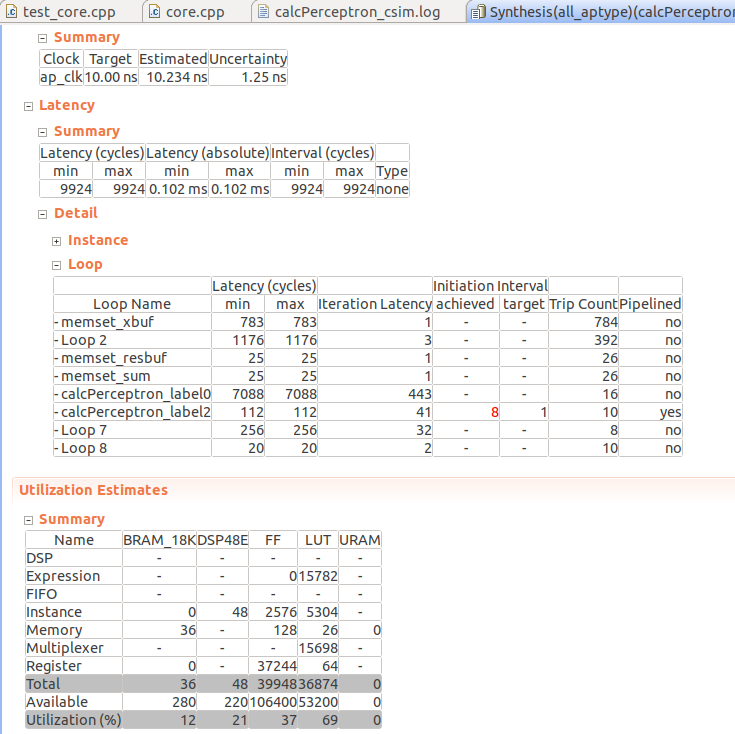
\includegraphics[width=\textwidth]{img/hls-report4.png}
  \caption{Raport po przeprowadzeniu syntezy w Vivado HLS -- minimalizowanie parametru II oraz redukcja zużycia zasobów}
  \label{hls-report4}
\end{figure}

Początkowo, implementację wykonano podając na blok HLS sygnał zegara o częstotliwości 250Hz. Jednak okazało się, że program nie działa poprawnie i po wykonaniu klasyfikacji jednego obrazu wchodził w stan zawieszenia. Po ustawieniu zegara na częstotliwość 100 MHz problem został rozwiązany i otrzymano poprawne wyniki. W wyniku syntezy otrzymano rozwiązanie wprowadzające niewielkie opóźnienia i akceptowalne zużycie zasobów. 
Wyeksportowano blok HLS do narzędzia Vivado i przeprowadzono syntezę i implementację projektu. Po wygenerowaniu Bitstreamu i eksporcie implementacji sprzętowej przetestowano rozwiązanie przy użyciu programu Vitis. Średni czas klasyfikacji jednej cyfry był ponad 7 razy krótszy niż w przypadku uruchomienia na CPU. Niestety spadła również dokładność klasyfikacji o~ponad 10\%. Wyniki przedstawiono w~Tabeli \ref{tab:czas-wykonania2}.

\begin{table}[h] \centering
  \caption{Porównanie czasu wykonania implementacji software'owej przy użyciu pakietu keras z~implementacją w układzie FPGA z wykorzystaniem akceleratora HLS -- po optymalizacji} 
  \centering
  \begin{tabular} {c|c|c|c} \hline \label{tab:czas-wykonania2}
      
      & czas wykonania & dokładność klasyfikacji & przyspieszenie obliczeń\\ \hline
     CPU & 0.516343 \emph{ms} & 91,6\%  & \\
     HLS & 0.070542 \emph{ms} & 81,0\% & 7.32$\times$ \\
    \end{tabular}
  \end{table}

